\section{format and use extisting partitions}
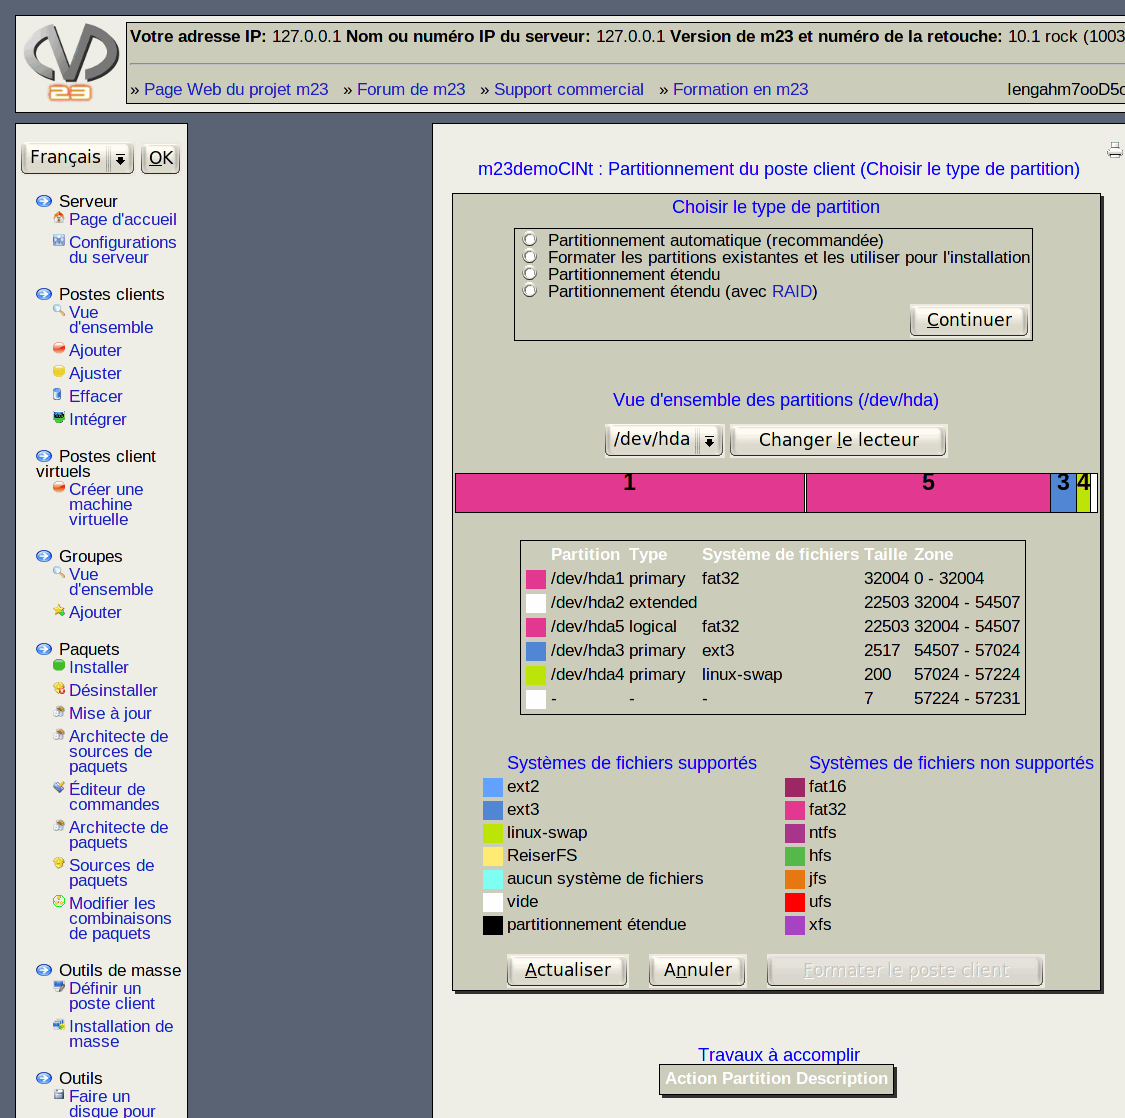
\includegraphics[scale=0.4]{/mdk/doc/manual/screenshots/en/fdisk-existing.png} \\
Here you have the possibility to reuse existing partitions. You have to select one partition for the base system and one for swapping.\\
\subsection{Step by step:}
\begin{enumerate}
\item Select \textit{"Format and use existing partitions"}.\\
\item Select the partitions you want to use for base system and swapping.\\
\item Click on the \textit{"Refresh"} button to see the partitioning.\\
\item Click on \textit{"Format client"} to accept changes.\\
\end{enumerate}
